% Provenance (never printed): cycle 3 "La planete Terre" and geography
% (weather and climate; reading a climate chart; the great climate zones of
% the world, hot, temperate and cold); see sources/book1/PROVENANCE.md.
% Book 1, grade 5, chapter 2.
\chapter{天气与气候}\label{ch:g5:weather-and-climate}

一月的第二周，学校收到两张明信片。
第一张来自莉娜的表亲，画面中孩子们在
阳光明媚的海滩上，棕榈树下堆沙堡。第二张来自汤姆的奶奶，
画面中孩子们在覆雪的花园里堆雪人。“同一周里，怎么会
既是夏天又是冬天？”汤姆问。

两地之间差异如此之大的，并不是某一天的\omterm{def:g1:watching-the-weather:weather}{天气}，
而是两地年复一年的\omterm{def:g1:watching-the-weather:weather}{天气}状况，即它们的\omterm{def:g5:weather-and-climate:climate}{气候}。

\begin{omfigure}
\begin{minipage}[b]{0.48\linewidth}\centering

\includegraphics[width=\linewidth]{images/book1/ai/g5-beach-postcard.jpg}
\end{minipage}\hfill
\begin{minipage}[b]{0.48\linewidth}\centering

\includegraphics[width=\linewidth]{images/book1/ai/g5-snowman-postcard.jpg}
\end{minipage}

{\small 一月同一周的两张明信片：阳光明媚的海滩和
覆雪的花园。}
\end{omfigure}

\begin{recall}
\omterm{def:g1:watching-the-weather:weather}{天气}是某地在某一时刻空气的状况：晴朗、
多云、下雨、下雪、刮风（见\cref{ch:g1:watching-the-weather}）。温度计
用来测量空气的温度，单位为摄氏度；\omterm{def:g4:clouds-rain-snow:rain-gauge}{雨量计}
用来测量降雨量，单位为毫米
（见\cref{ch:g4:clouds-rain-snow}）。\omterm{def:g3:continents-and-oceans:equator}{赤道}环绕\omterm{def:g3:continents-and-oceans:globe}{地球仪}的
中部，正好位于\omterm{def:g3:continents-and-oceans:poles}{北极}与\omterm{def:g3:continents-and-oceans:poles}{南极}之间。
（见\cref{ch:g3:continents-and-oceans}）。物理各册曾说明，
地球绕太阳公转一周需要一年，季节的变化来自
地轴的倾斜：夏季时，太阳在天空中升得更高，白天
也更长。
\end{recall}

\section{天气看今天，气候看平常}

\omterm{def:g1:watching-the-weather:weather}{天气}每天都在变化，甚至每小时都在变。\omterm{def:g5:weather-and-climate:climate}{气候}
则是另一回事。

\begin{definition}[气候]\label{def:g5:weather-and-climate:climate}
某地的\emph{气候}\index{气候}是指该地
通常出现的\omterm{def:g1:watching-the-weather:weather}{天气}，按月、多年统计：冷暖、
干湿如何，各季节的情况如何。气象学家通过对
30 年的测量数据取平均值来求得。
% ledger: wmo:normal-30yr
\end{definition}

“今天早上下雨”说的是\omterm{def:g1:watching-the-weather:weather}{天气}，“这里
秋天雨水很多”说的是\omterm{def:g5:weather-and-climate:climate}{气候}。夏天里的一个冷天
并不会改变\omterm{def:g5:weather-and-climate:climate}{气候}，它只是不寻常的\omterm{def:g1:watching-the-weather:weather}{天气}。

全世界的气象学家都采用同一规则：对
30 年的测量数据取平均值。目前所用的平均值
是 1991 年至 2020 年的数据。
% ledger: wmo:normal-30yr

\section{气候图}

为用一张图展示某地的\omterm{def:g5:weather-and-climate:climate}{气候}，需画出一张\omterm{def:g5:weather-and-climate:climate-chart}{气候图}。

\begin{definition}[气候图]\label{def:g5:weather-and-climate:climate-chart}
一张\emph{气候图}\index{气候图}展示一年中每个月
的平均气温（用一条曲线表示）和
该地降下的平均雨雪量（用柱表示，单位为毫米水柱）。
\end{definition}

\begin{omfigure}
\begin{tikzpicture}
  \begin{axis}[name=pax, width=0.55\linewidth, height=5.6cm, ymin=0, ymax=400,
      axis y line*=right, axis x line=none, ybar, bar width=7pt,
      ytick={0,100,...,400}, ylabel={降雨量 (mm)}, xmin=0.4, xmax=12.6,
      tick label style={font=\scriptsize}, label style={font=\scriptsize},
      ylabel style={blue!60!black}]
    \addplot[fill=blue!40, draw=blue!60!black]
      table[x=month, y=prcp_mm] {figdata/out/grade-5-climate_charts-seattle.dat};
  \end{axis}
  \begin{axis}[width=0.55\linewidth, height=5.6cm, ymin=-30, ymax=40,
      axis y line*=left, axis x line*=bottom, xmin=0.4, xmax=12.6,
      xtick={1,...,12}, xticklabels={1,2,3,4,5,6,7,8,9,10,11,12}, xlabel={月份},
      ytick={-30,-20,...,40}, ylabel={温度 ($^\circ$C)},
      tick label style={font=\scriptsize}, label style={font=\scriptsize},
      ylabel style={red!70!black}]
    \addplot[red!70!black, thick, mark=*, mark size=1.3pt]
      table[x=month, y=tavg_C] {figdata/out/grade-5-climate_charts-seattle.dat};
    \draw[gray!60] (axis cs:0.4,0) -- (axis cs:12.6,0);
    \begin{scope}[every node/.style={circle, draw, fill=white, inner sep=0.8pt,
        font=\scriptsize\bfseries}]
      \node[text=red!70!black, draw=red!70!black] at (axis cs:5.5,27) {1};
      \node[text=blue!60!black, draw=blue!60!black] at (axis cs:7,-19) {2};
    \end{scope}
  \end{axis}
  \node[anchor=north west, font=\scriptsize, align=left, text width=4.2cm]
    at ($(pax.outer north east)+(0.3,-0.1)$) {%
    \textcolor{red!70!black}{\textbf{1} 红色曲线：各月的平均温度
    ，在左侧刻度上读取。}\par\smallskip
    \textcolor{blue!60!black}{\textbf{2} 蓝色柱状：各月的平均降雨
    量，在右侧刻度上读取。}\par\smallskip
    \textbf{3} 图下方的数字：各月份，从一月
    到十二月。};
\end{tikzpicture}

{\small 西雅图的\omterm{def:g5:weather-and-climate:climate-chart}{气候图}。西雅图是位于美国
西\omterm{def:g1:landscapes-around-us:water}{海岸}的一座城市。图中数据为 1991 年至 2020 年的平均值（数据：NOAA）。}
% ledger: data:b1-noaa-normals
\end{omfigure}

\begin{method}[读懂气候图]\label{met:g5:weather-and-climate:reading}
\begin{enumerate}
  \item 在红色曲线上找出最暖和最冷的月份，
        并在左侧刻度上读出它们的温度。曲线是否平直（全年温度相同），
        还是有升有降（暖季与冷季）？
        还会降到 0~$^\circ$C 以下（霜冻）吗？
  \item 在蓝色柱状中找出降雨最多和最少的月份，
        并在右侧刻度上读出它们的降雨量。柱子是高是矮？
        是否有一段干燥的季节？
  \item 用一句话概括：“全年炎热干燥”，“温和湿润，
        夏季干燥”{\ldots}
\end{enumerate}
\end{method}

\begin{example}[西雅图]\label{ex:g5:weather-and-climate:seattle}
在西雅图，最暖的月份是八月（约 20~$^\circ$C），
最冷的是十二月（约 6~$^\circ$C）：曲线有升有降，
但从不降到冰点以下。最高的柱子是十一月的（约 160~毫米），
最矮的是七月的（约 15~毫米）。概括一句：冬季温和，夏季凉爽，
秋冬多雨，夏季较干。全年
降雨约 1\,000~毫米，相当于一米深的水层。
% ledger: data:b1-noaa-normals
\end{example}

\section{四种气候}

下面是美国四个彼此相距很远的城镇的\omterm{def:g5:weather-and-climate:climate-chart}{气候图}：
菲尼克斯位于亚利桑那州的\omterm{def:g5:weather-and-climate:desert}{沙漠}中；希洛位于太平洋中部的
夏威夷岛上；西雅图位于西\omterm{def:g1:landscapes-around-us:water}{海岸}；
乌特基亚维克位于阿拉斯加的最北端，濒临北冰洋。
四张图使用相同的刻度，因此可以一目了然地进行比较。

\begin{omfigure}
\def\gfivechart#1#2{%
\begin{tikzpicture}
  \begin{axis}[width=0.5\linewidth, height=4.6cm, ymin=0, ymax=400,
      axis y line*=right, axis x line=none, ybar, bar width=4pt,
      ytick={0,100,...,400}, xmin=0.4, xmax=12.6,
      tick label style={font=\tiny}]
    \addplot[fill=blue!40, draw=blue!60!black]
      table[x=month, y=prcp_mm] {figdata/out/grade-5-climate_charts-#1.dat};
  \end{axis}
  \begin{axis}[width=0.5\linewidth, height=4.6cm, ymin=-30, ymax=40,
      axis y line*=left, axis x line*=bottom, xmin=0.4, xmax=12.6,
      xtick={1,...,12}, xticklabels={1,2,3,4,5,6,7,8,9,10,11,12}, xlabel={月份},
      ytick={-30,-20,...,40}, tick label style={font=\tiny},
      title={#2}, title style={font=\scriptsize\bfseries, yshift=-4pt}]
    \addplot[red!70!black, thick, mark=*, mark size=1pt]
      table[x=month, y=tavg_C] {figdata/out/grade-5-climate_charts-#1.dat};
    \draw[gray!60] (axis cs:0.4,0) -- (axis cs:12.6,0);
  \end{axis}
\end{tikzpicture}}%
\gfivechart{phoenix}{菲尼克斯：炎热的\omterm{def:g5:weather-and-climate:desert}{沙漠}}\hfill
\gfivechart{hilo}{希洛：\omterm{def:g5:weather-and-climate:rainforest}{雨林}\omterm{def:g5:weather-and-climate:climate}{气候}}

\medskip
\gfivechart{seattle}{西雅图：温带\omterm{def:g5:weather-and-climate:climate}{气候}}\hfill
\gfivechart{utqiagvik}{乌特基亚维克：极地\omterm{def:g5:weather-and-climate:climate}{气候}}

{\small 四张\omterm{def:g5:weather-and-climate:climate-chart}{气候图}刻度相同：左侧为温度（红色曲线），
温度单位为 $^\circ$C；右侧为降雨量（蓝色柱状），单位为毫米。
图中数据为 1991 年至 2020 年的平均值（数据：NOAA）。}
% ledger: data:b1-noaa-normals
\end{omfigure}

\paragraph{\omterm{def:g5:weather-and-climate:desert}{沙漠}。}在菲尼克斯，柱子矮得
几乎看不见：全年降雨量不足 200 毫米。
夏季非常炎热：七月的平均温度是 35 摄氏度。
% ledger: data:b1-noaa-normals

\begin{definition}[沙漠]\label{def:g5:weather-and-climate:desert}
降雨极少的地方称为\emph{沙漠}\index{沙漠}，
即全年降雨量不足 250 毫米。那里很少有植物能够生存，
地面常常是裸露的。
% ledger: usgs:arid-250mm
\end{definition}

\omterm{def:g5:weather-and-climate:desert}{沙漠}并不总是炎热。看看乌特基亚维克：那里全年降雨
量不足 150 毫米，比菲尼克斯还少，这是一个寒冷的\omterm{def:g5:weather-and-climate:desert}{沙漠}。
\omterm{def:g5:weather-and-climate:desert}{沙漠}可以是炎热的，也可以是寒冷的。
% ledger: data:b1-noaa-normals, usgs:arid-250mm

\paragraph{\omterm{def:g5:weather-and-climate:rainforest}{雨林}。}希洛与菲尼克斯恰好相反。它的柱子
是四张图中最高的：全年降雨量超过 3\,000 毫米，
每个月都多雨。它的红色曲线几乎是平的：
全年在 22 至 25 摄氏度之间。这里根本没有冬季。
% ledger: data:b1-noaa-normals

\begin{definition}[雨林]\label{def:g5:weather-and-climate:rainforest}
由非常高大的树木组成的茂密森林称为\emph{雨林}\index{雨林}，
它生长在全年温暖湿润、每个月都有大量降雨的地方。
大多数雨林位于\omterm{def:g3:continents-and-oceans:equator}{赤道}附近。
\end{definition}

\begin{omfigure}
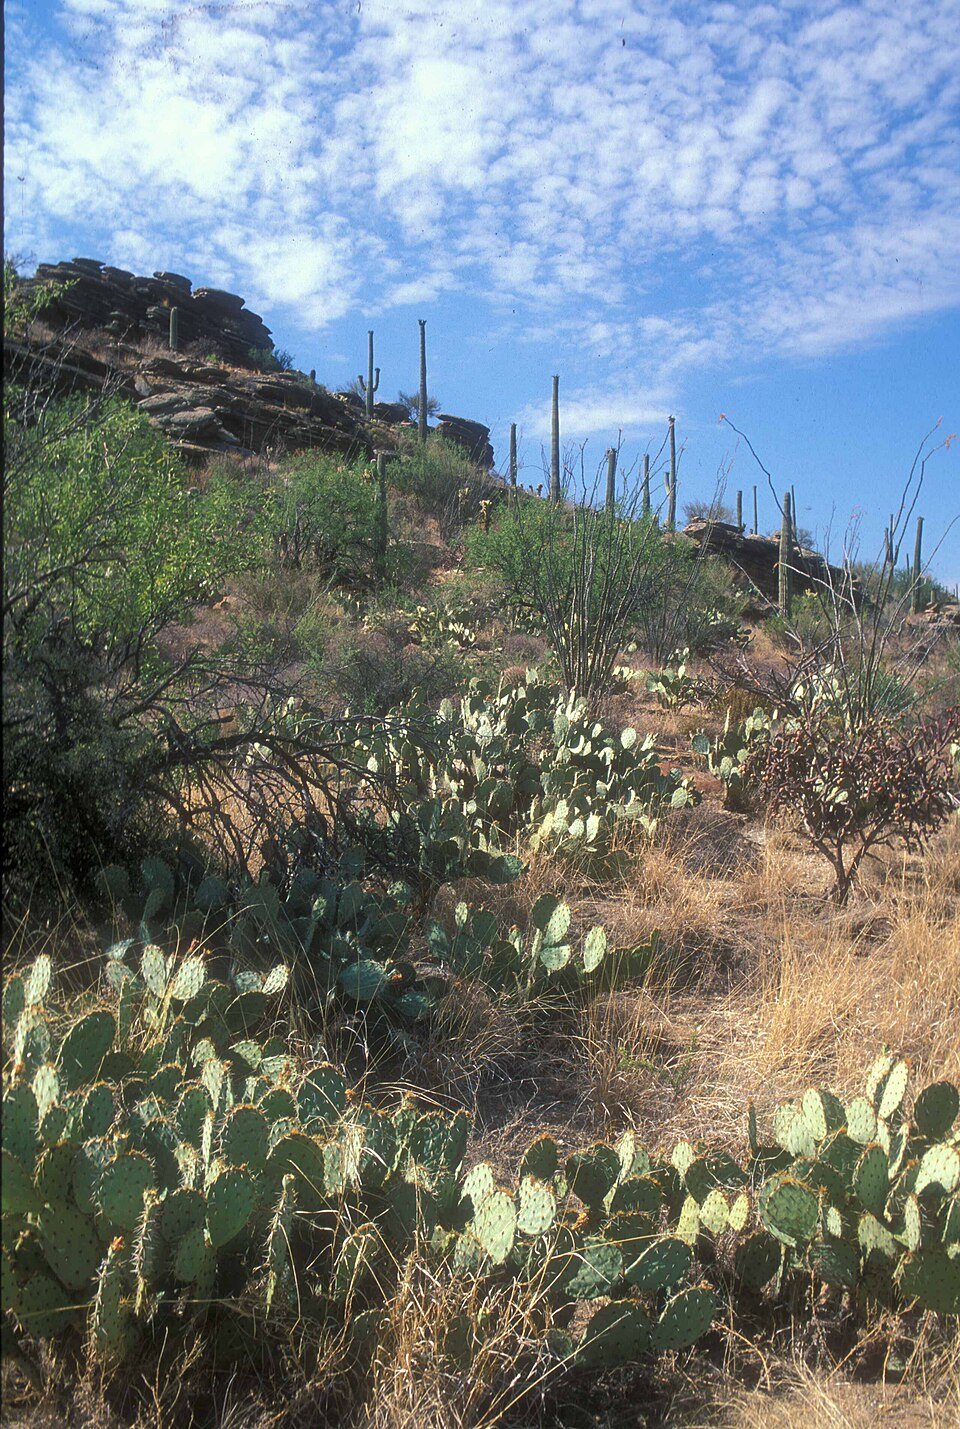
\includegraphics[height=3.6cm]{images/book1/g5-sonoran-desert.jpg}\quad
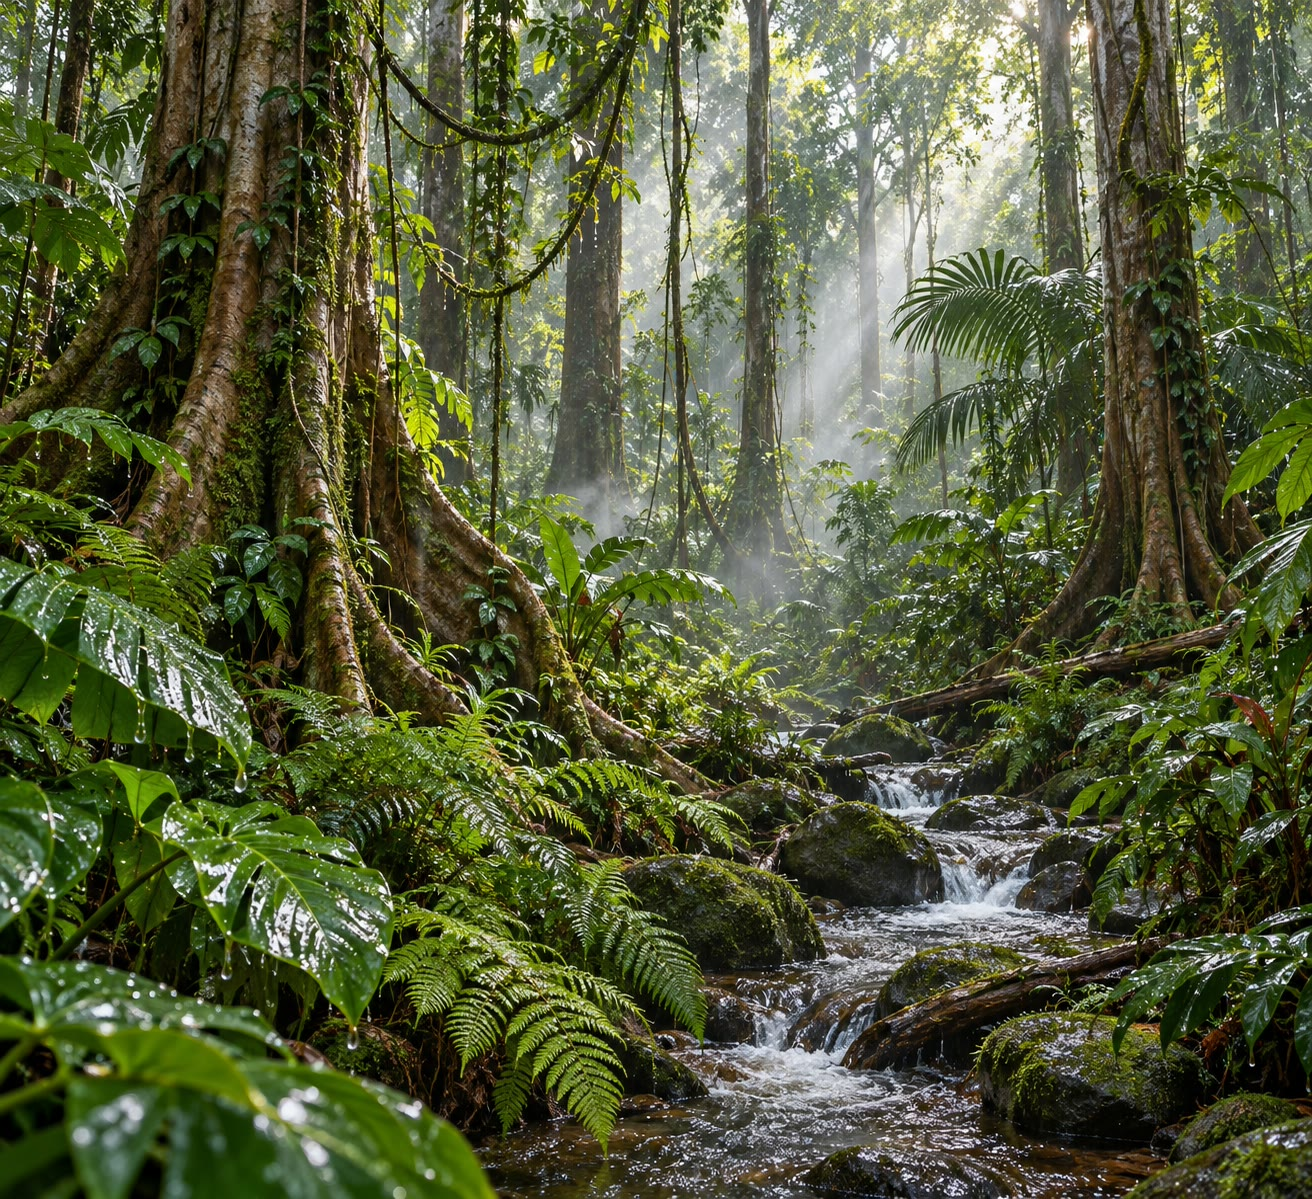
\includegraphics[height=3.6cm]{images/book1/ai/g5-rainforest.jpg}\quad
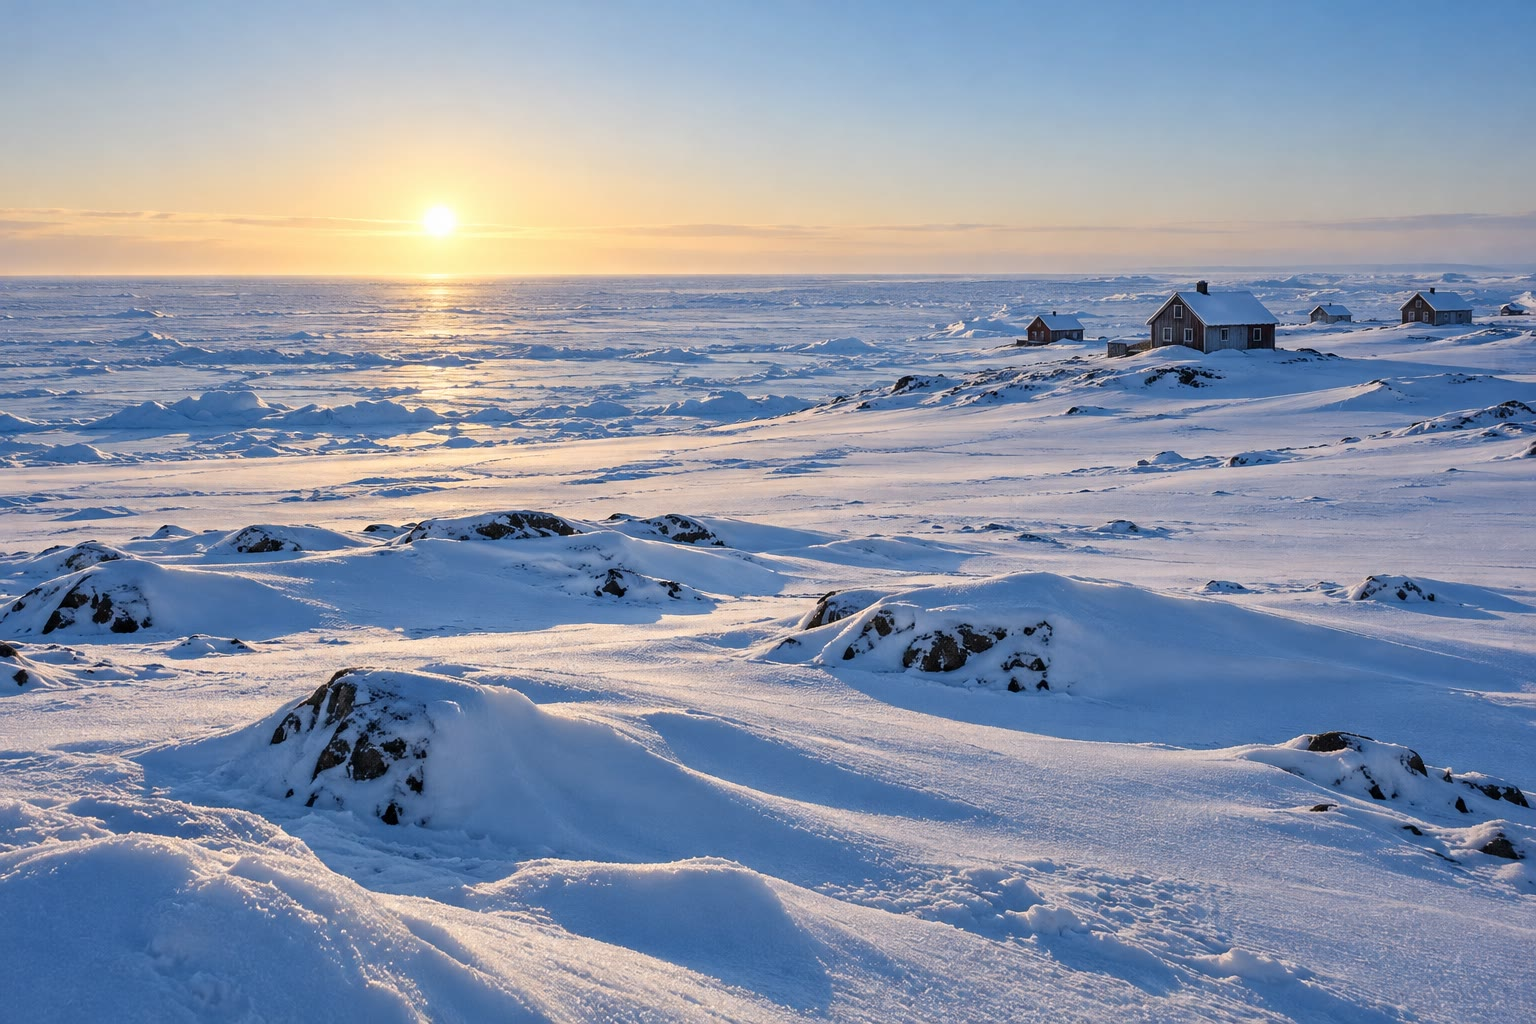
\includegraphics[height=3.6cm]{images/book1/ai/g5-polar-tundra.jpg}

{\small 三种极端\omterm{def:g5:weather-and-climate:climate}{气候}。左图：亚利桑那州的索诺兰\omterm{def:g5:weather-and-climate:desert}{沙漠}，即菲尼克斯所在的\omterm{def:g5:weather-and-climate:desert}{沙漠}，
那里生长着高大的巨人柱仙人掌和梨果仙人掌，它们的粗壮茎中储存着
水分（照片：U.S. National Park Service, Saguaro
National Park，公有领域）。中图：阵雨过后的\omterm{def:g5:weather-and-climate:rainforest}{雨林}内部。
右图：冬季的极地\omterm{def:g1:landscapes-around-us:water}{海岸}，海面结冰，正午时太阳很低。}
% ledger: nps:sonoran-desert
\end{omfigure}

\paragraph{温带\omterm{def:g5:weather-and-climate:climate}{气候}。}西雅图介于两者之间：它的曲线
夏季上升、冬季下降，但幅度从不太大；降雨量相当多，
主要集中在秋季和冬季。这是温带\omterm{def:g5:weather-and-climate:climate}{气候}：没有酷热，
也没有严寒。

\paragraph{极地\omterm{def:g5:weather-and-climate:climate}{气候}。}在乌特基亚维克，红色曲线全年有八个月低于
0~$^\circ$C；二月的平均气温为零下
24 度。即使在最暖的七月，平均气温也只有约
5 度。
% ledger: data:b1-noaa-normals

\section{热带、温带与寒带}

为什么\omterm{def:g3:continents-and-oceans:equator}{赤道}附近暖和，两极附近寒冷？这是因为
太阳。\omterm{def:g3:continents-and-oceans:equator}{赤道}附近，正午的太阳全年都高高地挂在天空中：
它的光几乎垂直照下来，使地面强烈升温。
两极附近，太阳始终很低：它的光斜着射来，
分散在很大的面积上，升温很少。那里的冬季，太阳
甚至可能整天不升起。

围绕地球的两对线把地球划分为不同的\omterm{def:g5:weather-and-climate:climate-zone}{气候带}。

\begin{definition}[回归线与极圈]\label{def:g5:weather-and-climate:tropics}
两条\emph{回归线}\index{回归线}是环绕地球的纬线，分别位于\omterm{def:g3:continents-and-oceans:equator}{赤道}以北和以南，
标出正午太阳能够直射头顶的最远位置：北面是北回归线，
南面是南回归线。两条\emph{极圈}\index{极圈}
是环绕地球的纬线，靠近两极，
越过它们的地方，在冬季正中
至少有一天太阳不升起；
在夏季正中太阳不落下：北面是\omterm{def:g3:continents-and-oceans:poles}{北极}圈，
南面是\omterm{def:g3:continents-and-oceans:poles}{南极}圈。
\end{definition}

地轴的倾斜决定了这些纬线的位置。

\begin{definition}[气候带]\label{def:g5:weather-and-climate:climate-zone}
地球被划分为三类\emph{气候带}\index{气候带}：位于两条\omterm{def:g5:weather-and-climate:tropics}{回归线}之间、环绕\omterm{def:g3:continents-and-oceans:equator}{赤道}的是\emph{热带}，
位于\omterm{def:g5:weather-and-climate:tropics}{回归线}与\omterm{def:g5:weather-and-climate:tropics}{极圈}之间、夏季与冬季有明显差异的是两个\emph{温带}，
位于\omterm{def:g5:weather-and-climate:tropics}{极圈}之外、
环绕两极的是两个\emph{寒带}。
\end{definition}

\begin{omfigure}
\begin{tikzpicture}
\begin{axis}[ommap, width=\linewidth, xtick=\empty, ytick=\empty, grid=none,
    axis background/.style={fill=white}, clip=true]
  \addplot[fill=orange!35, draw=none] table {figdata/out/grade-5-climate_zones-hot.dat};
  \addplot[fill=green!20, draw=none] table {figdata/out/grade-5-climate_zones-temperate.dat};
  \addplot[fill=cyan!20, draw=none] table {figdata/out/grade-5-climate_zones-cold.dat};
  \addplot[fill=black!25, fill opacity=0.8, draw=black!60, line width=0.2pt]
    table {figdata/out/shared-geo-land.dat};
  \addplot[black!70, dashed, line width=0.5pt] table {figdata/out/grade-5-climate_zones-lines.dat};
  \draw[black!70, line width=0.6pt] (axis cs:-180,0) -- (axis cs:180,0);
  \addplot[only marks, mark=*, mark size=1.8pt, red!80!black]
    table[x=lon, y=lat] {figdata/out/grade-5-climate_zones-stations.dat};
  \begin{scope}[every node/.style={font=\scriptsize, fill=white, fill opacity=0.75,
      text opacity=1, inner sep=1pt}]
    \node[anchor=west] at (axis cs:-107,33.4) {凤凰城};
    \node[anchor=east] at (axis cs:-158,19.7) {希洛};
    \node[anchor=west] at (axis cs:-117,47.4) {西雅图};
    \node[anchor=west] at (axis cs:-151,73.5) {乌特基亚维克};
  \end{scope}
  \begin{scope}[every node/.style={font=\scriptsize\bfseries, align=center,
      fill=white, fill opacity=0.7, text opacity=1, inner sep=1pt}]
    \node at (axis cs:-5,83) {寒带};
    \node at (axis cs:-40,40) {温带};
    \node at (axis cs:-25,-8) {热带};
    \node at (axis cs:95,-45) {温带};
    \node at (axis cs:-60,-80) {寒带};
  \end{scope}
\end{axis}
\end{tikzpicture}

{\small \omterm{def:g5:weather-and-climate:climate-zone}{气候带}。从上到下，虚线依次是\omterm{def:g3:continents-and-oceans:poles}{北极}圈、北\omterm{def:g5:weather-and-climate:tropics}{回归线}、南\omterm{def:g5:weather-and-climate:tropics}{回归线}和
\omterm{def:g3:continents-and-oceans:poles}{南极}圈；实线是\omterm{def:g3:continents-and-oceans:equator}{赤道}。红点是
上方\omterm{def:g5:weather-and-climate:climate-chart}{气候图}中的四个
城镇。}
% ledger: earth:obliquity, data:b1-noaa-normals
\end{omfigure}

\omterm{def:g5:weather-and-climate:climate-zone}{气候带}只给出一个初步的粗略图景。在每个\omterm{def:g5:weather-and-climate:climate-zone}{气候带}内部，还有许多其他因素
影响\omterm{def:g5:weather-and-climate:climate}{气候}：一个地方离海多远、地势多高、风从何处来。这些内容你将在
以后的年级学到。

\begin{remark}[凤凰城与气候带]\label{rem:g5:weather-and-climate:phoenix}
在\omterm{def:g5:weather-and-climate:climate-zone}{气候带}\omterm{def:g2:drawing-to-map:map}{地图}上，凤凰城位于北\omterm{def:g5:weather-and-climate:tropics}{回归线}略偏北的地方，
属于温带，然而它是一个炎热的\omterm{def:g5:weather-and-climate:desert}{沙漠}。\omterm{def:g5:weather-and-climate:climate-zone}{气候带}只是
初步的粗略图景：许多大型热\omterm{def:g5:weather-and-climate:desert}{沙漠}位于\omterm{def:g5:weather-and-climate:tropics}{回归线}附近，
处在热带的边缘，你将
在\cref{ch:g8:winds-global-circulation}中了解其中的原因。
\end{remark}

\section{练习}

\begin{exercise}[$\star$]\label{exo:g5:weather-and-climate:1}
是\omterm{def:g1:watching-the-weather:weather}{天气}还是\omterm{def:g5:weather-and-climate:climate}{气候}？
\begin{enumerate}
  \item[(a)] 今天早晨乌特基亚维克正在下雪。
  \item[(b)] 在凤凰城，夏季非常炎热干燥。
  \item[(c)] 昨天下午西雅图刮起了大风。
  \item[(d)] 在希洛，每个月都下很多雨。
\end{enumerate}
\end{exercise}

\begin{exercise}[$\star$]\label{exo:g5:weather-and-climate:2}
某地的\omterm{def:g5:weather-and-climate:climate}{气候}是什么？\omterm{def:g1:watching-the-weather:weather}{天气}学家要对多少年的测量数据取平均，
才能描述该地的\omterm{def:g5:weather-and-climate:climate}{气候}？
\end{exercise}

\begin{exercise}[$\star$]\label{exo:g5:weather-and-climate:3}
在西雅图的\omterm{def:g5:weather-and-climate:climate-chart}{气候图}上，哪个月最冷？
哪个月降雨最多？气温是否曾低于 0~$^\circ$C？
\end{exercise}

\begin{exercise}[$\star$]\label{exo:g5:weather-and-climate:4}
在乌特基亚维克的\omterm{def:g5:weather-and-climate:climate-chart}{气候图}上，哪个月最暖和？
是否有哪个月的气温高于 10~$^\circ$C？
\end{exercise}

\begin{exercise}[$\star$]\label{exo:g5:weather-and-climate:5}
说出下列各地点分别位于哪个\omterm{def:g5:weather-and-climate:climate-zone}{气候带}：\omterm{def:g3:continents-and-oceans:equator}{赤道}、\omterm{def:g3:continents-and-oceans:poles}{北极}，
以及\omterm{def:g3:continents-and-oceans:equator}{赤道}与\omterm{def:g3:continents-and-oceans:poles}{南极}之间中途的某一地点？
\end{exercise}

\begin{exercise}[$\star$]\label{exo:g5:weather-and-climate:6}
利用\omterm{def:g5:weather-and-climate:climate-zone}{气候带}分布图，判断下列四个城镇各位于哪个\omterm{def:g5:weather-and-climate:climate-zone}{气候带}：
凤凰城、希洛、西雅图、乌特基亚维克？
\end{exercise}

\begin{exercise}[$\star\star$]\label{exo:g5:weather-and-climate:7}
下表给出西雅图各月的平均降雨量（单位：毫米），
数值已取整数：
\begin{center}
\begin{tabular}{|*{12}{c|}}
\hline
J & F & M & A & M & J & J & A & S & O & N & D\\
\hline
147 & 96 & 106 & 81 & 48 & 37 & 15 & 25 & 41 & 99 & 160 & 145\\
\hline
\end{tabular}
\end{center}
西雅图一整年的降雨量是多少？
12 月、1 月和 2 月这三个月共降雨多少？
% ledger: data:b1-noaa-normals
\end{exercise}

\begin{exercise}[$\star\star$]\label{exo:g5:weather-and-climate:8}
凤凰城的平均气温：1 月为 14~$^\circ$C，
7 月为 35~$^\circ$C；希洛的平均气温：1 月为 22~$^\circ$C，
7 月为 25~$^\circ$C。分别计算两地 7 月与 1 月的气温差，
并判断哪个地方的气温随季节变化更大？
% ledger: data:b1-noaa-normals
\end{exercise}

\begin{exercise}[$\star\star$]\label{exo:g5:weather-and-climate:9}
下表给出某虚构城镇的各月平均值。
\begin{center}
\begin{tabular}{|l|*{12}{c|}}
\hline
月份 & J & F & M & A & M & J & J & A & S & O & N & D\\
\hline
气温（$^\circ$C） & 27 & 27 & 28 & 28 & 28 & 27 & 27 & 27 & 27 & 27 & 27 & 27\\
\hline
降雨量（mm） & 250 & 230 & 280 & 290 & 260 & 180 & 170 & 160 & 190 & 230 & 250 & 260\\
\hline
\end{tabular}
\end{center}
该城镇属于\omterm{def:g5:weather-and-climate:desert}{沙漠}\omterm{def:g5:weather-and-climate:climate}{气候}、\omterm{def:g5:weather-and-climate:rainforest}{雨林}\omterm{def:g5:weather-and-climate:climate}{气候}、温带\omterm{def:g5:weather-and-climate:climate}{气候}还是极地\omterm{def:g5:weather-and-climate:climate}{气候}？请给出两条理由；
它最可能位于哪个\omterm{def:g5:weather-and-climate:climate-zone}{气候带}？
\end{exercise}

\begin{exercise}[$\star\star$]\label{exo:g5:weather-and-climate:10}
回看本章开头的两张明信片，它们是在同一个一月的同一周寄出的。
请给出两种不同的解释，说明为什么孩子们在一个地方可以在晴朗的海滩上玩耍，
而在另一个地方却在堆雪人。
\end{exercise}

\begin{exercise}[$\star\star\star$]\label{exo:g5:weather-and-climate:11}
诺尔说：“凤凰城和西雅图都位于温带，
所以它们的\omterm{def:g5:weather-and-climate:climate}{气候}一定相同。”请利用\omterm{def:g5:weather-and-climate:climate-chart}{气候图}说明她的说法是错误的：
比较两地的气温和降雨。然后说明\omterm{def:g5:weather-and-climate:climate-zone}{气候带}告诉了我们什么，
以及没有告诉我们什么。
\end{exercise}
